%!TEX root = ../INTO-CPS-Manifesto.tex

\section{The INTO-CPS Tool Chain}\label{sec:toolchain}

This section discusses the interconnectivity of the different tools, and how the tools fit into the workflows and tasks that are covered by INTO-CPS. In particular, this section focuses on the features that were added during the INTO-CPS project, and in the framework of the INTO-CPS association. This section does \textit{not} describe all the tools in detail (here, the reader is referred to the different manuals, and to the User Manual \cite{INTOCPSD4.3a} and to Appendix \ref{appendix:tools}). The main concepts of the tool-chain are discussed above in Section \ref{sec:method:concepts}.

An overview of the different tools that form the tool-chain of the INTO-CPS association, is given below in Figure \ref{fig:fulltool-chain}, where the red boxes indicate the different sections of this chapter.

\begin{figure}[!ht]
	\centering
		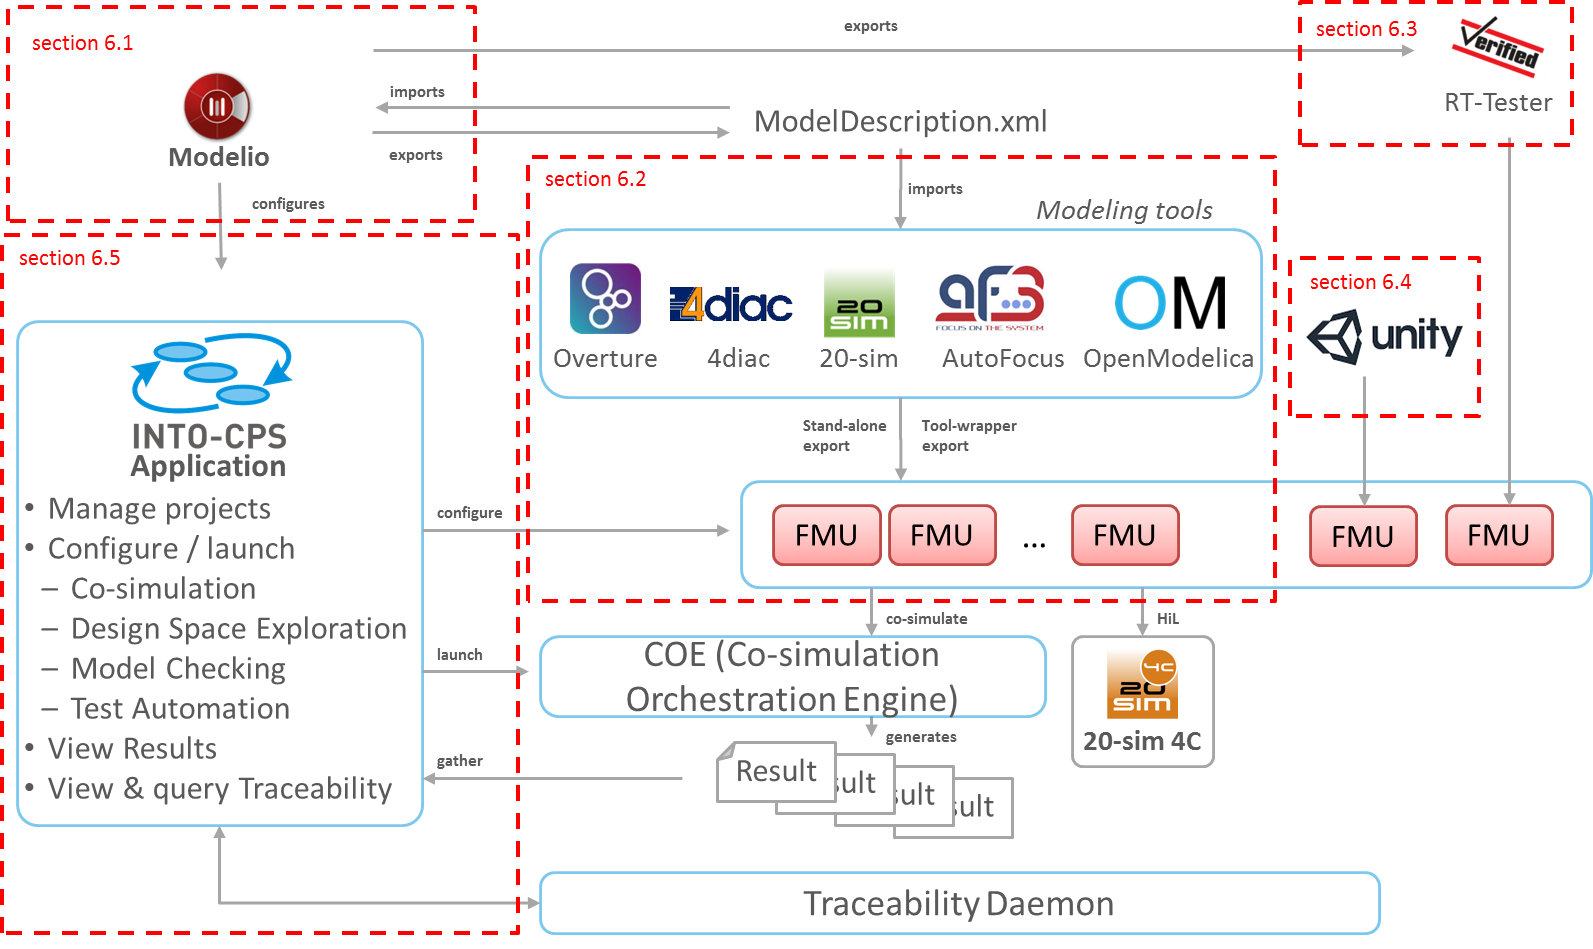
\includegraphics[width=0.9 \textwidth]{./figures/toolchain_association}
	\caption{Overview of the different tools and their arrangement in a tool-chain.}
	\label{fig:fulltool-chain}
\end{figure}
%[Figure of the overall tool-chain]

\subsection{Modelio}
\label{sec:modelio}
Modelio is an open-source modelling environment for various formalisms with many interfaces to import and export models. In the context of INTO-CPS, the support for SysML modelling is of primary importance, while Modelio can be extended with a range of modules to enable more modelling languages. In the terminology of the methods guidelines (e.g.\ \cite{Pierce&18}), Modelio is a tool for the \textit{architectural modelling} and for \textit{requirements management}.

During the INTO-CPS project, a SysML profile was created, which is currently available as a module for Modelio 3.4 and 3.6\footnote{see \url{http://forge.modelio.org/projects/intocps}}. This INTO-CPS SysML profile extends Modelio with several functionalities that described in detail elsewhere \cite{INTOCPSD41c,INTOCPSD4.2c,INTOCPSD4.3c}. Here, only those parts of the INTO-CPS SysML profile are discussed that add features for interconnectivity in the tool-chain.

To support the FMI multi-modelling approach, \texttt{ModelDescription.xml} files can now be imported into, and exported from a SysML Architectural Modelling diagram. Importing \texttt{ModelDescription.xml} files creates a SysML block with the corresponding flow ports and attributes, exporting them allows import in other modelling tools, such as those described below in Section \ref{sec:toolchain:tools}.

The Connections Diagram describes the signal flow between the different SysML blocks, which can each correspond to one FMU. Using the INTO-CPS SysML profile, the Connections Diagram can be exported to an intermediary JSON format, which can then be imported by the INTO-CPS Application, to create a new Multi-Model.

Diagrams for handling of Design Space Exploration (DSE) were created for Modelio, also included in the INTO-CPS SysML profile. These diagrams allow connection of parameters with signals, definition of objectives for a DSE, connection of signals with objectives, and ranking of results. Using these diagrams, a complete DSE configuration can be exported from Modelio.

Behavioural models that are designed in Modelio as state machines can be exported as \texttt{.xmi} files, so that they can be imported to the RT Tester tool.

Furthermore, Modelio allows Requirements management, and supports traceability in the context of INTO-CPS. More details about Modelio can be found in Section~\ref{app:modelio}.

\subsection{Modelling tools}
\label{sec:toolchain:tools}

At the core of the tool-chain are several modelling tools that describe a system or a sub-system in a specific formalism, and perform calculations to understand the dynamic behaviour of the (sub-)system. While the formalisms or application areas can be vastly different, the modelling tools share some common features, which are summarised in this section.

\paragraph{20-sim} is a commercial tool for modelling and simulation of mechatronic systems. Together with the related software, 20-sim 4C, Hardware-in-the-Loop simulations can be performed (\url{http://www.20sim.com/}). This is described further in Section~\ref{app:20sim}.

\paragraph{OpenModelica} is an open-source environment which is based on the Modelica language. It features numerous free libraries to easily model systems from different domains (\url{https://openmodelica.org/}). This is described further in Section~\ref{app:OM}.

\paragraph{Overture} is an open-source tool that supports the modelling method \textit{The Vienna Development Method (VDM)}, which is a formal method to describe computing systems (\url{http://overturetool.org/}). This is described further in Section~\ref{app:overture}.

\paragraph{4Diac} is an open-source tool for distributed process measurement and control systems based on the IEC 61499 standard\footnote{See \url{https://www.eclipse.org/4diac/}.}. This is described further in Section~\ref{app:4diac}.

\paragraph{AutoFocus3} is an open-source model based tool to develop embedded software systems. \url{https://af3.fortiss.org/}

%\paragraph{Cossim}

\paragraph{ABS} is a language for Abstract Behavioural Specification, which combines implementation-level specifications with verifiability, high-level design with executability, and formal semantics with practical usability. ABS is a concurrent, object-oriented, modelling language that features functional data-types. \url{http://abs-models.org/}

Most modelling tools support the same functions in the context of INTO-CPS. A \texttt{ModelDescription.xml} file (e.g.\ one that is automatically created from Modelio, see previous section) can be imported to create a skeleton model with the input and output signals and exposed parameters. After the actual modelling work is done, the model can be exported as Functional Mock-up Unit (FMU), in accordance with the FMI 2.0 for Co-Simulation standard. This FMU can either contain all the necessary models and solvers, so that is a self-contained model (also called stand alone), or it contains libraries which call a simulation tool to execute the simulation. The latter case is called a tool wrapper FMU. Furthermore, the different steps of importing, saving and exporting generate traces which are sent to the traceability engine of the INTO-CPS Application. The following table summarises the status of the different tools at the time of writing of this document.

\begin{table*}[ht]
	\centering
		\begin{tabular}{|l|p{1.7cm}|p{1.7cm}|p{1.7cm}|p{1.7cm}|p{1.7cm}|}\hline
			\rotatebox[origin=c]{90}{Tool} & \rotatebox[origin=c]{90}{MD.xml import} & \rotatebox[origin=c]{90}{FMU import} & \rotatebox[origin=c]{90}{FMU export (stand alone)} & \rotatebox[origin=c]{90}{FMU export (tool wrapper)} & \rotatebox[origin=c]{90}{Traceability}\\
			\hline
			20-sim & yes & yes & no & yes & yes\\ \hline
			OpenModelica & yes & yes & yes & no & yes\\ \hline
			Overture & yes & yes & yes & yes & yes\\ \hline
			4diac & no & no & yes & no & no \\ \hline
			AutoFocus 3 & no & under development & no & no & no\\ \hline
			%Cossim & N.A. & N.A. & N.A. & N.A. & N.A. \\
			ABS & no & no & no & planned & no \\ \hline
		\end{tabular}
	\caption{Functionalities of the modelling tools}
	\label{tab:FunctionalitiesOfTheModelingTools}
\end{table*}

\subsection{RT Tester}
\label{sec:tool-RTTester}

In the framework of INTO-CPS, the RT Tester tool suite (see \url{https://www.verified.de/products/rt-tester/}) is extended with mainly two objectives: Integration of Test-Automation and of Model Checking in the INTO-CPS tool-chain. Both functions are integrated into the INTO-CPS application, and both support traceability. This is described further in Section~\ref{app:RTT}.

\subsubsection{Test Automation}

Test Automation within INTO-CPS uses the RT Tester tools to generate, perform and analyse tests, based on Co-simulation of a system. The Test Automation functionalities are integrated into the INTO-CPS Application. The behavioural model can be generated in Modelio, and exported as \texttt{.xmi} file, which in turn can be read by RT Tester. After the test is created in RT Tester, the test procedure can be cast into an FMU file. Together with a Co-Simulation scenario, and using the COE, the test procedure is used to run a test project. More information on Test Automation in INTO-CPS can be found in \cite{INTOCPSD5.3b}.

\subsubsection{Model Checking}

Model checking in INTO-CPS is used to verify system properties of multi-models, consisting of continuous-time (CT) and discrete-event (DE) models. Similar to the Test Automation features, Model Checking is based on the RT Tester tool suite. From a tool-chain perspective, Model Checking is integrated in the INTO-CPS Application, which allows the complete configuration, execution and analysis of a Model Checking experiment. More information on Model Checking in INTO-CPS can be found in \cite{INTOCPSD5.3c}.


\subsection{3D animation}

The 3D animation FMU allows visualisation of the simulation. It is based on the Unity engine (see \url{https://unity3d.com}), and extends it by exporting the scenario and the 3D rendering as a FMU \cite{Foldager&17}. The Modelio SysML profile (see Section \ref{sec:modelio}) takes the visualisation FMU into account. The 3D animation FMU also supports Virtual Reality (VR) headsets. The source code for this is available for the members of the INTO-CPS Association in a special SVN.

\subsection{The INTO-CPS Application}

The INTO-CPS Application is the central tool to integrate the different tools and artefacts, to configure and run simulations, manage results, and more. It allows configuration and execution of DSE scenarios (which can be imported from Modelio), and is a front-end for Model-checking and Test automation, by using the RT Tester tool (see Section~\ref{sec:tool-RTTester}). Furthermore, traceability data can be viewed in the Application, either in an expert view, using the Neo4J visualisation\footnote{\url{https://neo4j.com/}}, or by pre-configured queries. 